\chapter{System Overview}

\section{Architectual structure}

\begin{figure}[h!]
    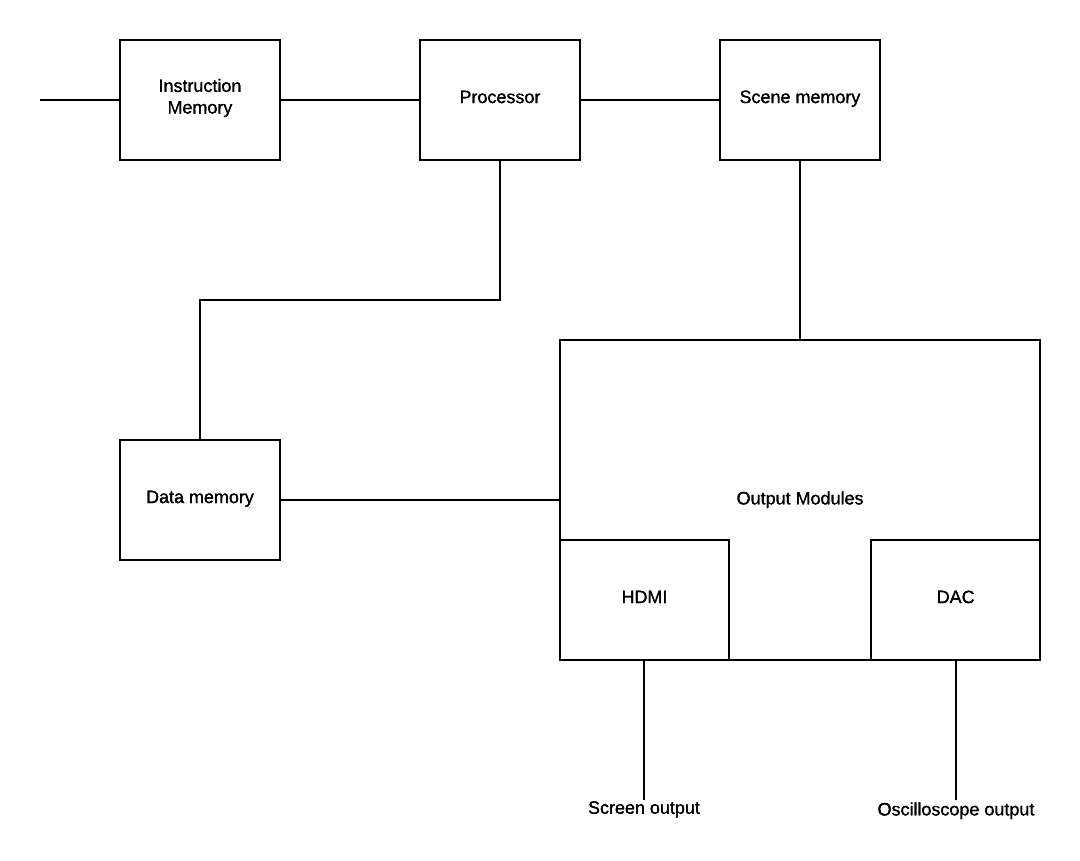
\includegraphics[width=\linewidth]{images/system-overview.png}
    \caption{A logical overview of the \vthreek architecture}
    \label{fig:system-overview}
\end{figure}

Figure \ref{fig:system-overview} shows how the major building blocks of the \vthreek architecture come together on a conceptual level.
Separation of instruction and data memory makes it a Harvard-like architecture.
The processor reads from instruction memory, executes instructions and adds/updates vector primitives in the scene memory.
Preprocessing these primitives for output is done by the output modules.
For the HDMI output, this involves rasterizing each primitive and maintaining a framebuffer.
The oscilloscope output is generated by serializing primitives onto two DACs.

\section{Programming Model}

The \vthreek architecture is fairly conventional and largely RISC-inspired.
This makes its programming model fairly similar to that of other modern computers.

A .v3k program is assembled on a host machine, transferred to the microcontroller which in turn loads it into instruction memory.
As previously mentioned, the \vthreek architecture is general, and as such, offers support for integer arithmetic, load/store instructions and simple branching.
Additionally, instructions for adding and processing vector primitives such as lines and curves are available.
A complete description of the \vthreek ISA is available in appendix \ref{app:ISA}.

\subsection{A Simple \vthreek Program}

\begin{lstlisting}[label=lst:simple-program]
mov r1, #0
lsl r1, r1, #16
mov r1, #0

mov r2, #65535
lsl r2, #16
mov r2, #65535

line r1, r2
strp #0x00000001
\end{lstlisting}

Listing \ref{lst:simple-program} shows a very simple \vthreek program.
It simply draws a line across the scene, from bottom left corner to top right.

Vector primitives consist of a varying number of integer numbers.
In the case of a line, it consists of four 16-bit coordinates.
To utilize registers effectively, each 32-bit register is loaded with one x,y coordinate-pair.

The first three lines put the coordinates $0,0$ in register \texttt{r1}, the next three puts $65535$ in register \texttt{r2}.
The values in the registers are then used to create a line starting at \texttt{r1} and ending at \texttt{r2}.
Finally, the line is written to the scene memory using \texttt{strp}.

Upon creating a primitive with \texttt{line}, \texttt{bezquad} or \texttt{bezqube}, the resulting primitive is stored in a special purpose register in the processor.
To actually add the primitive to the scene, it has to be written to the scene memory using \texttt{strp}.
Primitives can also be loaded from the scene to be modified or processed using \texttt{ldrp}.
Only one primitive can be active in the processor at a time.
